\documentclass[12pt]{article}
\usepackage{parskip}
\usepackage[nottoc]{tocbibind}
\usepackage{url}
\usepackage{float}

% center captions
\usepackage{caption}
\captionsetup{justification=centering}

% code
\usepackage{xcolor}
\usepackage{inconsolata}
\usepackage{xpatch}
\usepackage{realboxes}

\definecolor{numcolour}{HTML}{757575}
\definecolor{codegreen}{HTML}{428747}
\definecolor{backcolour}{HTML}{EDEDED}
\definecolor{codebrown}{HTML}{A34900}

\usepackage{listings}
\lstset{basicstyle=\ttfamily}

\lstdefinestyle{yaml}{
    numberstyle=\color{numcolour}\footnotesize\ttfamily,
    basicstyle=\color{black}\footnotesize\ttfamily,
    backgroundcolor=\color{backcolour},
    comment=[l]{\#},
    commentstyle=\bfseries\color{codegreen},
    string=[s]{"}{"},
    stringstyle=\color{codebrown},
    breaklines=true,
    numbers=left,
    showstringspaces=false,
    frame=single,
    captionpos=b
}

\lstdefinestyle{http}{
    numberstyle=\color{numcolour}\footnotesize\ttfamily,
    basicstyle=\color{black}\footnotesize\ttfamily,
    backgroundcolor=\color{backcolour},
    comment=[l]{>},
    commentstyle=\color{codebrown},
    breaklines=true,
    showstringspaces=false,
    frame=single,
    numbers=left,
    captionpos=b
}



% highlighting
\usepackage{color}
\usepackage{soul}

% images
\usepackage{graphicx}
\graphicspath{ {./img/} }

\begin{document}

    \makeatletter
    \xpretocmd\lstinline{\Colorbox{backcolour}\bgroup\appto\lst@DeInit{\egroup}}{}{}
    \makeatother

    \begin{titlepage}
        \begin{center}
            \vspace{1cm}

            \LARGE
            Electronics and Computer Science\\
            Faculty of Physical Sciences and Engineering\\
            University of Southampton\\

            \Large
            \vspace{1.5cm}
            \textbf{Augustas Mirinas}\\
            \today

            \LARGE
            \vspace{1.5cm}
            \textbf{Trustless System for Personal Data Sharing}
            
            \vspace{1.5cm}
            \Large
            Project supervisor: Dr George Konstantinidis\\
            g.konstantinidis@soton.ac.uk
            
            \Large
            Second examiner: Dr Mark Vousden\\
            m.vousden@soton.ac.uk
            
            \vfill
            A project report submitted for the award of\\
            BSc Computer Science
            
        \end{center}
    \end{titlepage}

    \section*{Abstract}
    

    \newpage
    \tableofcontents

    
    \newpage
    \section{Introduction}
    Many modern companies and organizations provide online services, making internet user data more abundant and valuable than ever. Collected user information is utilised to run tailored advertising and promotions, improve customer experience or facilitate research by providing useful statistics. In this setting collected personal data has become a valuable asset which can be traded and shared. This, however, comes with a serious privacy issue - after sharing their information, data subjects lose control over it, which is a natural problem of centralised information exchanges. Most online service users will have a choice to consent to data processing. This choice, however, indicates user consent only in the context of that online service, and is useless when taking malicious organizations into consideration. An organization ignoring user consent can collect all user information available, without any evidence of breaching user consent. Information can then be shared to an unknowing party, who can only trust the publisher, because there is no way to independentely validate information legitimacy. This section will hypothesize the requirements to solve this problem of trust.

    \subsection{Trustless system}
    The goal of this project is to create a trustless system for personal data sharing. Trustless system reffers to a system, comprised of actors, untrusting of each other, but united by the same benefits of the system. A member of the system is encouraged to follow data privacy rules, because it can observe and confirm whether other members also follow data privacy rules. If a malicious system member ignored consent policies, other members would be able to notice it and revoke malicious member access to the system. This decentralised approach to information exchange, its benefits and challenges are considered in \cite{dlt}. This publication states "key benefits for adopting blockchain technology in biomedical and health care applications include: decentralized management, immutable audit trail, data provenance, robustness/availability, and security/privacy."\cite{dlt} These factors divide personal data control equally between every information exchange member, also generating a trace of data usage which can be examined to validate transactions of data. Some challenges been highlighted as well: confidentiality and scalability - natural problems for blockchain technology. Considering these findings, the main requirement of a trustless system is (1) decentralisation. However, for decentralised system to be practical and comparable to a centralised information exchange approach, it must have (2) scalable data storage with permissioned access to confidential information as well.

    \subsection{User consent}
    Decentralised information exchange solves the problem of trust, defeating third-party intervention in progress: cryptocurrency is independent from any institution, therefore no institution can reverse a cryptocurrency payment. This can be a problem in the context of personal data exchange, because the project aims to (3) keep data subjects in full control of their data. This requirement, paired with decentralisation, means that data subjects should be participants of the decentralised system in some way. Section \ref{sec:literature} will discuss whether they should be represented by a trusted organization, or complete part of computing for the decentralised system. User consent is also a design problem, deciding how should personal data consent be expressed and controlled. Solution for this problem is adapted from \cite{konstantinidis}, published by the supervisor of this project.
    
    \subsection*{Project scope}
    This project is aimed to design and implement a working prototype of an information exchange, which does not base data privacy on trust. The report focuses on the ability to share personal information, complying with data sharing consent at the same time. This project report is assuming basic knowledge on blockchain and some understanding around smart contracts.

    
    \section{Literature review}
    \label{sec:literature}
    A number of decentralised healthcare information systems are reviewed and their features compared in this section. The results are used to model an information exchange that best solves the problems introduced earlier. This section will focus on the degree of control given to the user, as well as data storage solutions of each system reviewed.

    \subsection{Consent management}
    Tackling a similar problem of personal data ownership, \cite{privacy} proposes digital signatures as a way to confirm authorised access to personal data. This is achieved by running a blockchain network to store users identities and implement access logic. Identities are sets of public and private keys, and can be validated by the blockchain network. This network also stores user access policies, which express identities with access to different subsets of user data. Then, blockchain network is used as an information exchange to upload and query shared data in the system. The user is always in full control of their policies and can revoke them at any time, which satisfies a requirement for data sharing consent. Furthermore, every interaction is recorded into the ledger, ensuring transparency and safe data usage.

    Another publication about personal data ownership \cite{gateways}, delegates the authorization of each personal data query up to the user. The purpose of the system proposed is to be a confidential and secure health information exchange, where data subjects are in full control of their data. Healtcare practitioners request access to patient data for more accurate diagnosis or treatment, and patients decide whether to share requested information or not. Access to shared information can be given temporarily - only for the duration required by the practitioner. This system, similar to above, utilises identities validated by the blockchain to authorise data querying and updating operations. Another shared feature is blockchain network as an intermediary between information publishers and the system storage - here, blockchain immutability is used to ensure every member respects personal data.

    While both systems had given the user control over their information, consent to share personal data is expressed more efficiently in \cite{privacy}. Having to approve or reject every query might create a bottleneck when receiving batch requests from multiple users. Storing user consent once and using it to process query data, on the other hand, is a much more efficient way to ensure personal data privacy. The algorithm defines data sharing consent semantics as a set of permissions, because mobile application authorisation is based on giving permissions. These are simple semantics, well-suited for mobile environment. For a more general information exchange design, an algorithm from \cite{konstantinidis} is used to define consent semantics. This section also discovered that such network requires access logic to be independently executed by the blockchain network. 
    
    Distributed execution is achieved by multiple members simulating the same task with the same input, and agreeing on the result of that simulation. After executing a function on the blockchain network, transaction is generated as an output, recording the change of the public ledger state. The block is signed by multiple network participants and is appended to the public ledger. A node, honestly maintaining the public ledger, is assigned to verify transactions invoked by other members and is able to invoke transactions itself. Therefore, system members have a common interest to keep the public ledger up to date, making blockchain network transparent and independent.

    \subsection{System attributes}
    For a decentralised network, storage implementation is also an important decision. System, proposed in \cite{privacy}, introduces encryption as a way to store raw data without compromising it. Published data is stored off-chain, invisible to blockchain network. However, network ledger contains pointers to a distributed hashtable. To read or write personal data, a correct identity must be presented in order to update the hashtable via blockchain - decrypting table data and managing access is computed independently, based on the implemented blockchain protocol. This results in data storage, where all access rules are in the blockchain system, every execution being approved by the majority of participants and no single actor has control on all data stored in the system, because the storage is split into multiple components, each storing only part of all data.

    A safety threat, natural to public blockchain networks, is a 51\% attack on a blockchain. If new blocks are approved by the majority of nodes, a malicious actor controlling 51\% of blockchain computation power would have the ability to approve invalid blocks. The solution to this problem is a permissioned blockchain, as described in \cite{permissioned}. Approved healthcare institutions, research laboratories and other authorized actors would form a distributed ledger. Interactions with patient data are recorded in the ledger by a smart contract. To implement this immutable and permissioned ledger,  publication proposes segmented system governance - verifier entity authenticates system users, and consensus nodes confirm new blocks. There is a third entity: issuer registering new users. No entity out of three has the ability to approve invalid transactions without others' approvals. In result, transactions in the system are now confirmed by a consortium of selected and trusted members. This design still prevents single-point failure, at the same time disallowing invalid transaction submition from unapproved participants.

    From publishings like \cite{dlt} and others reviewed in this section, it is clear that a blockchain system is very efficient at distributing control over all network participants. However, computation required for transaction approval and ledger broadcasting would make it unusable when facing frequent and bigger requests in practice, due to storage limits and response times. Clear solution is to use off-chain data storage, not replicated on any network node. This storage would only be accessible via blockchain, and any request to read/write must be authenticated and authorised by system policies, implemented on the public ledger. Off-chain storage may be deployed to a private cloud, or possibly an off-grid distributed storage, similar to IPFS\cite{ipfs}. Nevertheless, no system reviewed in this section specified what could be the actual actors managing the blockchain system. An example of implementation could have countries, contributing some computing nodes to form an authority of personal data protection. Other implementations could design each data subject responsible for their data only. To conclude, decisions of system design may be based on metrics - update frequency, data volume, speed and scalability requirements and privacy concerns. In further sections, single implementation will be finalised to reach the objectives of this project.


    \section{Design}

    \subsection{Information exchange}
    \label{subsec:design:exchange}

    % data publishing
    This information exchange achieves data privacy using an algorithm to compute "consent-abiding query answers" from the publication of the supervisor of this project \cite{konstantinidis}. In this publication, to ensure that parts of private data, not consented to share, will stay private, data queries are rewritten in compliance with data subject constraints. These constraints consist of rules specifying data tuples that are prohibited from sharing. Each data subject has their own set of constraints, which is used as neccessary when rewriting data queries. After rewriting, resulting queries would only return data that is consented for sharing. By project definition, the algorithm would be executed in a trustless environment, therefore it is assumed system members would try re-identification - an exploit to identify a data subject by matching results from multiple different queries. To adapt consent semantics of \cite{konstantinidis} for this problem, information published to this system is filtered before saving it on the system, instead of saving raw data and rewritting queries of that data. All user consent is used when publishing information to upload only data that the user has consented to share. Network participants must use existing consent expressions to get data upload transaction approved. This is the basic logic of consent-abiding information exchange, whose members are not required to be trusted, as data during uploading is filtered by the system, not by the publisher.

    % filtering and constraints
    In order to publish private information, it has to be linked to an existing user (data subject). If a subject of published data does not exist, the information will not be saved to the system. To create a user identity, data subject must come up with a unique system username and submit it through an independent party, possibly a government body or other data protection authority. In this design, external authority was selected as a provider for user identification. User control over personal data has not been challenged, however, because the authority has no access to system data. Similarly to \cite{permissioned}, this design distributes validation role to different members every transaction, and an external party is responsible for new block approval and broadcasting. After issuing new user identity, consent constraints can be defined using an index of the information as a reference - the data is published in the form of a table, which enables expressing consent constraints as combinations of table columns. This results in a simple, but powerful consent definition, which can be used to prevent user re-identification.

    % index and table format
    Both constraints and the index of data conforms to the table format. A single constraint is expressed as a combination of columns from the index - some examples with explanation can be seen in Figure \ref{fig:constraints}, which is taken from \cite{konstantinidis}. The data being published contains records, or rows, with a username column to specify which user this record belongs to. The index, defining all columns of the record, is already created at the time of setting a new constraint. Only then can the data about this user, collected by some organization, be published to the system allowing authorised members of the network to access it, without compromising data subject's consent. By referencing an existent table index, user is certain their consent meaning will not change, because the table index is final. Table format makes data format less flexible, but the table schema is essential for applying consent constraints and saving the right information.

    \begin{figure}[H]
        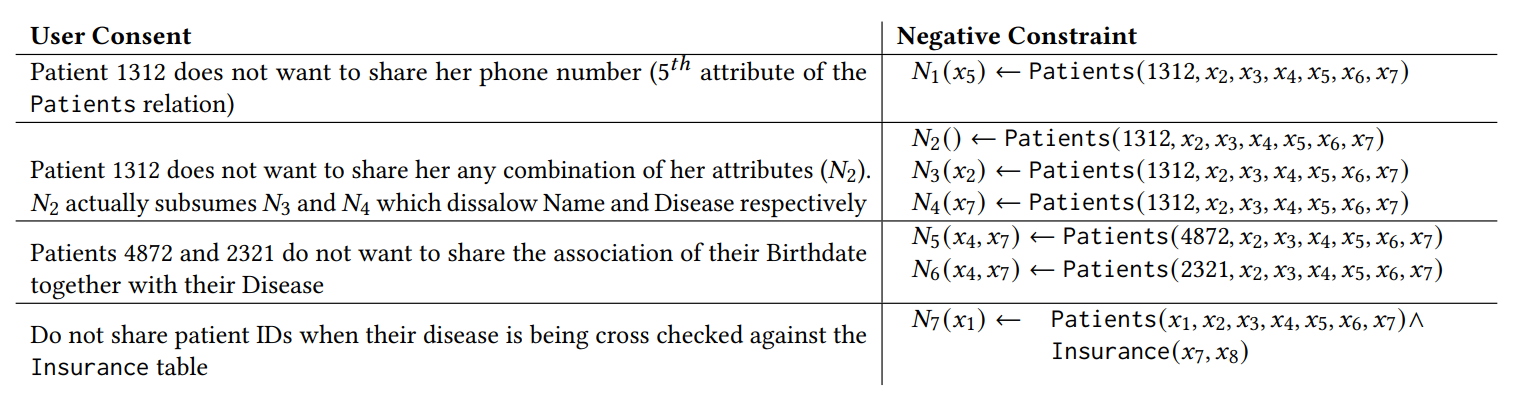
\includegraphics[width=\textwidth]{constraints.png}
        \caption{A capture of the table showing some examples of user constraint semantics}
        \label{fig:constraints}
    \end{figure}


    \subsection{Distributed architecture}
    Traditionally, sensitive user information for sharing is pooled into a single place, then accessed by different parties as needed. However, this approach requires trusted organization with complete control over all private information. The design chosen for this project relies on blockchain technology - utilising decentralisation and immutability to create a system, where shared information cannot be manipulated and is maintained by every permissioned member of the network. Components of the system are distributed across contributors of the network, and every network member is identified and approved. In this arrangement, data storage and information processing is a collective effort of all members, dependant on every participant. Centralised data stores also present a trade-off between data availability and required space. In case of corrupt data, archives of databases need to be kept, however this comes with increased system size. A decentralised blockchain network addresses data availability by having up-to-date replicas on multiple machines. This also increases system size the same way archives do, but one machine will only store information that is actively used, drasticaly reducing the upper size limit for a single data store.

    Active members of the network - nodes - represent data publishing or exchanging organizations. Nodes store information  they have access to and approve new transactions, maintaining the network in collaboration. Curiously, common incentive to maintain a public ledger is the strongest when all members get similar level of benefits from the system. For example, 4 members, each share their data to one member, and read data from a different member. The common incentive to keep up the system ledger is strong, compared to a system where one member is sharing data to other three members, without receiving data themselves. This situation would not create any incentive to participate in the blockchain as a publishing member. Balance of benefits could potentialy be used to assess the level of motivation each network has to maintain its public ledger.
    
    % blockchain ledger
    To enforce the network policies on the participants, the system produces a record of every network member interaction. These records, containing information about the interaction and ordered based on the interaction timestamp, form a public ledger. Member interactions with the system are also called transactions. Only transactions, approved by required members are valid and recorded into a ledger. The ledger is replicated across multiple network members to prevent any unauthorised changes to the ledger - if a malicious member would attempt to change the record of system transactions, other network members would still be able to agree on the correct ledger version and deny the unauthorised change, based on their ledger replicas. This results in a system that consists of multiple independent members following the same rules and policies. This feature of the blockchain network is used for implementation of the data privacy algorithm presented in subsection \ref{subsec:design:exchange}.
    
    % decentralised data storage
    One major advantage of a blockchain network over a traditional centralised information exchange approach is data storage. The proposed blockchain network does not store data on the ledger, nor does it communicate private information through transactions - meaning actual data intended for sharing is never recorded on the public ledger. Instead, when publishing new data to the system only the hash of data is made public. Actual private data is stored only by the data publisher and any members that have access to it. This model records evidence of published data and makes it public to everyone without revealing the contents of published data. By inspecting hashes of data in the ledger, it is possible to confirm private data was not tampered with after publishing. This and more scenarios will be analysed in section \ref{sec:scenario}. Another benefit of fragmented data storage is damage mitigation in case of a data breach or a malicious access. A member of the network will only store information that is either used or published by themselves - in most cases this will be a small subset of overall private data published to the system, which means a single instance of a data breach would compromise less private information than in the traditional centralised data exchange, where all private information is pooled to a single place.
    
    Cloud storage is a legitimate consideration for this system as well. First thing to decide when considering a data sharing system is the storing of information. Most standard way to store information is cloud-based services. Cloud storage requires minimal setup and no maintenance of on-premise databases, it also has practically unlimited space and the price for this service depends on the amount of information stored - meaning this solution is highly scalable. Given cloud storage would be only accessible via the blockchain, secure access logic will preserve personal information confidentiality. This design will not have a cloud storage, because data stored in cloud relies on the cloud service provider, which violates the decentralisation requirement. In case of cloud service outtage, shared data would be unavailable. In the end, this decision depends on the context and nature of shared information.
    
    \subsubsection{Components}
    The blockchain network implementing this design is permissioned, meaning every member of the network is known and has defined access to resources and permissions to validate certain transactions. This is different from public blockchain systems, such as Bitcoin\cite{bitcoin} or Ethereum\cite{ethereum}, where unknown members can be part of the network and their transactions are validated via "proof of stake" or other consensus mechanisms. In this system, the task of transaction validation is designated to a trusted provider of this service - a member of the network with the role of deciding which transactions have correct signatures and should be recorded into the ledger. This, however, does not include signing the transactions - each member of the system retains responsibility of signing valid transactions. Nodes can also issue identities - certifications that are used for identification and authentication. These identities can be used to give access to query the system via blockchain functions, or register a new data subject to set constraints. To have this service, every member must deploy a certificate authority (CA) - a node issuing identities for this network member. Many identities can exist at the same time, with different roles and attributes. Access can be based on identities attributes - meaning different individuals, while having access to the same network member, may have different access level on the network. With the implementation of a permissioned network, the system can utilise identitities to create more expressive access information access policies.
    
    The component to implement after the network validator is a channel. This network component defines which network members are able to participate in the channel, how transactions of the channel should be approved and who can make and approve changes to the channel configurations, which may vary depending on the use case of this system. Current design gives control of system logic to data subjects. For each channel, a set of functions are defined in smart contracts of the blockchain network. These functions implement private data filtering using user constraints and enable data publishing, reading and constraint registering. Furthermore, smart contracts define collections of data and which members can read or write to those collections. These network components allow highly customizable segmentation of information access. Different areas of information can be separated into channels - each one would have an individual ledger, resulting in smaller chunks of isolated data.

    Any participant of this system can interact with it via their node, however, some users interested in utilising this system may not be able to have an active node in the network. Data subject, for example, is a single person without a technical knowledge about blockchains. It would be a mistake to assume this person is able to connect their personal computing device to the network and be a part of the ledger. To solve this issue, each member of the system can deploy an application with correct connection profile, to act as a gateway between the user and the blockchain network. This additional software layer can invoke transactions, select what members to ask for transaction approval, receive blockchain events and query the public ledger. It may seem the application defeats the purpose of decentralisation, as each member just has a version of application, which only they control. However, the blockchain gateway is only an interface - the backend logic of the system is still dictated by the collective of all permissioned network nodes.
    
    \section{Implementation}
    
    To implement this blockchain system for secure and consent-abiding private data sharing Hyperledger Fabric will be used - an "open source enterprise-grade permissioned distributed ledger technology platform"\cite{fabric}. This technology was established under the Linux Foundation, which has a reputable history of open source projects. Hyperledger Fabric is a permissioned blockchain system, meaning every member of the network knows each other. This is well suited for a proposed design, as all members - either data subjects or data publishers - should be approved anyway. Every member of the system has the same goal - provide useful information or use it for a good cause. Any action is recorded on a ledger, deterring any malicious members to take action and face consequences.

    \subsection{Environment and tools}
    \label{subsec:environment}
    The deployment of this implementation is not production grade - to ease development process, explanation of the system and to allow easy replication for anyone interested, all network components are deployed on a single machine. Docker Compose is used for this purpose - by defining a \lstinline{docker-compose.yaml} file, multiple containers are brought up using officialy supported Docker images and Hyperledger Fabric commands. These commands use environment variables and generated network certification files to correctly set up nodes of the network. In production environment, these files and variables should be carefully considered and stored in different machines of each component of the network, but in this project the Docker Compose configuration and other required files are going to be generated by Fablo - "a simple tool to generate the Hyperledger Fabric blockchain network"\cite{fablo}. Fablo takes one configuration file as an input and generates the network with specified organizations and other neccessary settings, files and components. Then \lstinline{fablo} commands can be used to manage the generated network. This tool is part of Hyperledger Labs - a space to start and contribute to projects related to Hyperledger Fabric, which guarantees official Hyperledger support and compatibility. Another tool with the same origin is Blockchain Explorer\cite{explorer}, useful for observing transactions made on the network using graphical user interface. Java with Maven is used for developing smart contracts and Git for version control.

    \subsection{Network configuration}
    \label{subsec:network}
    In Hyperledger Fabric, the node validating blockchain network transactions is called an orderer. Here, orderer is hosted by a regulating authority - a trusted organization interested in securing private user data. It is also responsible for data subjects' identities - because every Fabric network user must be identified and authorised, this trusted organization gives out identities for users to use when submiting consent constraints, which will be used to only publish information consented for sharing, while information unrelated to any constraint is discarded. Other three organizations are separate business entities, publishing private data collected from users (data subjects). Each organization is only a logical unit; to interact with the network, each organization has one physical network node, called peer in Hyperledger Fabric. As stated in subsection \ref{subsec:environment}, network configuration files and required environment variables will be generated with the help of Fablo, therefore in this section Fablo configuration file will be demonstrated, which is more concise and easier to explain compared to many files, required for the Fabric network. Here, only a part of the configuration file will be shown with comments to explain each setting.

    \begin{lstlisting}[style=yaml,
        caption={fablo.yaml - configuration file generating the network}, label={lst:network}]
---
# global network settings
global:
    fabricVersion: "2.5.0"
    # enable TLS for secure communication between network nodes
    tls: true
    tools:
        # start a Node.js server hosting Blockchain Explorer
        explorer: true
orgs:
    # data publisher or consenter organization
  - organization:
        name: "Org1"
        mspName: "Org1MSP"
        domain: "org1.co"
    # certificate authority settings - node issuing organization identities
    ca:
        prefix: "ca"
    peer:
        prefix: "peer"
        # multiple nodes could be used to have multiple data points in the organization
        instances: 1
        db: "LevelDb"
    tools:
        # enable REST interface to call chaincode and create identities
        fabloRest: true

    # ...
    # two more organizations are defined but omitted with identical settings
    # org2.ac
    # org3.gov
    # ...
    
    # trusted authority organization, hosting a node which validates transactions
  - organization:
        name: "Owners"
        mspName: "OwnersMSP"
        domain: "owners.org"
    ca:
        prefix: "ca"
    peer:
        prefix: "peer"
        instances: 1
        db: "LevelDb"
    orderers:
      - groupName: "authority",
        prefix: "orderer",
        type: "raft",
        # can be more than one orderers for redundancy
        instances: 1
    tools:
        fabloRest: true
    
channels:
    # one channel consisting of all organizations defined
  - name: "ch1"
    orgs:
        - name: "Org1"
        peers:
            - "peer0"
        - name: "Org2"
        peers:
            - "peer0"
        - name: "Org3"
        peers:
            - "peer0"
        - name: "Owners"
        peers:
            - "peer0"
chaincodes:
    # ...
    \end{lstlisting}

    After generating the network using given configuration in listing \ref{lst:network}, all nodes are created and started. As mentioned, each organization has its own peer, which can interact with the network. Organization \lstinline{mspName} can be used to control resource access in smart contracts - this is used when granting access to create consent constraints for \lstinline{owners.org} organization. Another option for organization is database implementation. Every node has an instance of database, where network data, such as consent constraints or published user information, is stored and queried from. Any changes in network data is propagated in databases of each node. Option \lstinline{db} specifies whether to use LevelDb or CouchDb for peer database implementation. LevelDb is used for this project, utilising its flexibility and speed. Data is stored as ordered key-value pairs, and maps string keys to byte array values, meaning any information can be stored, as long as it can be deterministically serialized into bytes. CouchDb is a NoSQL database storing data as JSON objects, which runs as a separate database process and enables rich queries, however it is left for future considerations. Lastly, a single channel is defined consisting of peers of every organization defined. In figure \ref{fig:network}, all spawned Docker containers and Hyperledger Fabric commands used to start them are shown.
    
    \begin{figure}[H]
        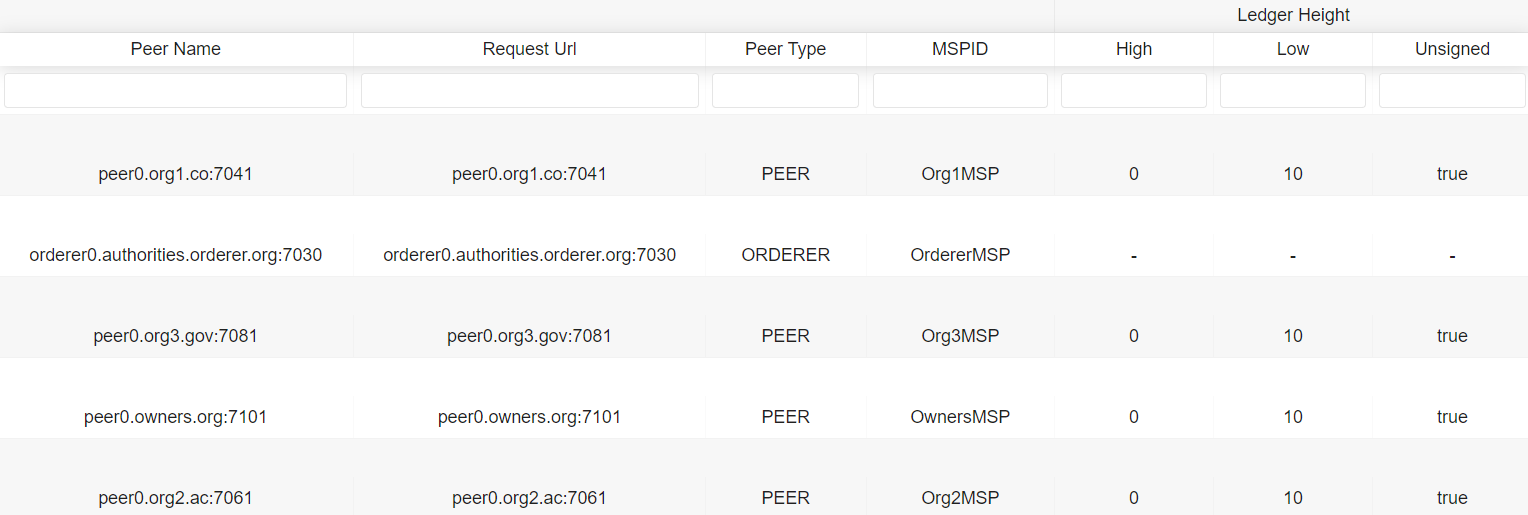
\includegraphics[width=\textwidth]{network.png}
        \caption{A Blockchain Explorer table listing all network components}
        \label{fig:network}
    \end{figure}


    \subsection{Chaincode endorsement}
    In figure \ref{fig:network}, ledger height can also be seen. The largest number corresponds to 10 blocks appended to the ledger. These blocks contain transactions, which are produced with \lstinline{peer lifecycle chaincode} commands, which install chaincode to the Fabric network. Chaincode defines smart contracts, which have a set of functions, that describe what actions can be executed in the network. These transactions are used to setup the network, and more transactions may be produced by updating, installing or invoking the chaincode. For different organizations to use the same chaincode, the correct version of packaged smart contracts must be agreed by the administrators of organizations.
    
    Every chaincode has an endorsement policy, indicating which organizations have to approve transactions produced by chaincode invokes. To facilitate endorsement each endorsing organization executes invoked function on their own peer node and sends the output of the function to the ordering service. If all required peers agree on the same output, the orderer writes function output to the ledger and all channel peers update their instance of the ledger to the newest version. Endorsement policies are agreed at the time of chaincode installation and they are applied for every chaincode invoke. In Fablo, network chaincode with endorsement policies is also defined in the configuration file from listing \ref{lst:network}. In listing \ref{lst:chaincode}, a continuation of \lstinline{fablo.yaml} is shown.

    \begin{lstlisting}[style=yaml,
        caption={fablo.yaml - configuration file defining network chaincode}, label={lst:chaincode}]
---
global:
    # ...
orgs:
    # ...
channels:
    # ...
chaincodes:
  - name: "private-data"
    version: "1.0"
    # language that the chaincode is written in
    lang: "java"
    # channel that will have this chaincode installed
    channel: "ch1"
    # physical directory of the chaincode files
    directory: "private-data-chaincode"
    endorsement: "OutOf(2, 'OwnersMSP.member', 'Org1MSP.member', 'Org2MSP.member', 'Org3MSP.member')"
    # private data collections shared with different organizations to controll private information access
    privateData:
      - name: "CollectionA"
        orgNames:
            - "Org1"
            - "Org3"
      - name: "CollectionB"
        orgNames:
            - "Org1"
            - "Org2"
            - "Org3"
      - name: "CollectionC"
        orgNames:
            - "Org2"
            - "Org3"
    \end{lstlisting}

    The chaincode in Hyperledger Fabric is installed to one channel only, meaning other channels in the system will have their own version of chaincode, with different endorsement policies and collections. Endorsement policies make the network transparent - a chaincode invoke is impossible without the knowledge of other endorsing members and the result of the invoke is agreed by all endorsers. Separate channels, however, give the ability to select a specific set of functions, collections and an endorsement policy based on the sensitivity and usage of shared data, as well as relations between channel organizations.

    In this implementation, option \lstinline{endorsement} defines a policy - transactions have to be endorsed by two out of four existing organizations. One endorsing organization is not enough, as an organization could submit invalid chaincode invoke and endorse it itself - meaning user data could be published with consent constraints bypassed. Other limitation of endorsing organizations is a concern of data privacy. When endorsing a chaincode invoke, uncensored data is submited as an input and censored based on network consent constraints during chaincode execution. Endorsing node temporarily stores submitted input to emulate the chaincode and sign the output, during which time sensitive information can be read. To combat this problem, in production deployment channels should contain significantly more organizations compared to endorsers. For instance - in a channel with 30 organizations and an endorsing policy of three organizations, each one would have the ability to use this exploit once in every ten transactions - which would not yield any significant advantage over other organizations. Furthermore, there is a possibility to manually choose which organizations are chosen for endorsement, and require for \lstinline{Owners} organization to endorse every publishing transaction - this way exposing sensitive information to a trusted organization only. This will be further explained in section \ref{sec:future}.

    \subsection{Private collections}
    In listing \ref{lst:chaincode} option \lstinline{privateData} defines collections and organizations with access to them. In this network configuration, each of the three data publishing organizations have access to two or three private collections. \lstinline{owners.org} does not get any access, because it does not publish, nor read data from the system - only submit consent constraints. Private data published on the system will be written into one of three collections implemented as replicated data stores, separate from the public channel ledger, which are maintained only by organizations with access to that collection - one organization maintains three ledgers: one public ledger and two private collections, except \lstinline{org3.gov}, which has access to all collections. Even with limited access to collections, every organization can stil emulate write-only transactions, as these invokes do not rely on having access to private data. Endorsement of transactions involving writing and querying from a private collection is only done by organizations with sufficient access - meaning \lstinline{owners.org} can only endorse read invokes from the public ledger. Figure \ref{fig:collections} contains all network nodes with a channel ledger and accessible private collections. Arrows indicate communication - thicker arrows are public transactions of the channel, issued by the orderer for every change of the ledger. Remaining arrows represent gossip between peers with access to private collections. These updates are not public and does not use orderer as a verifier, since collection updates do not produce transactions. This way data remains uncompromised, but still agreed on by multiple nodes hosting collection data.
    
    \begin{figure}[H]
        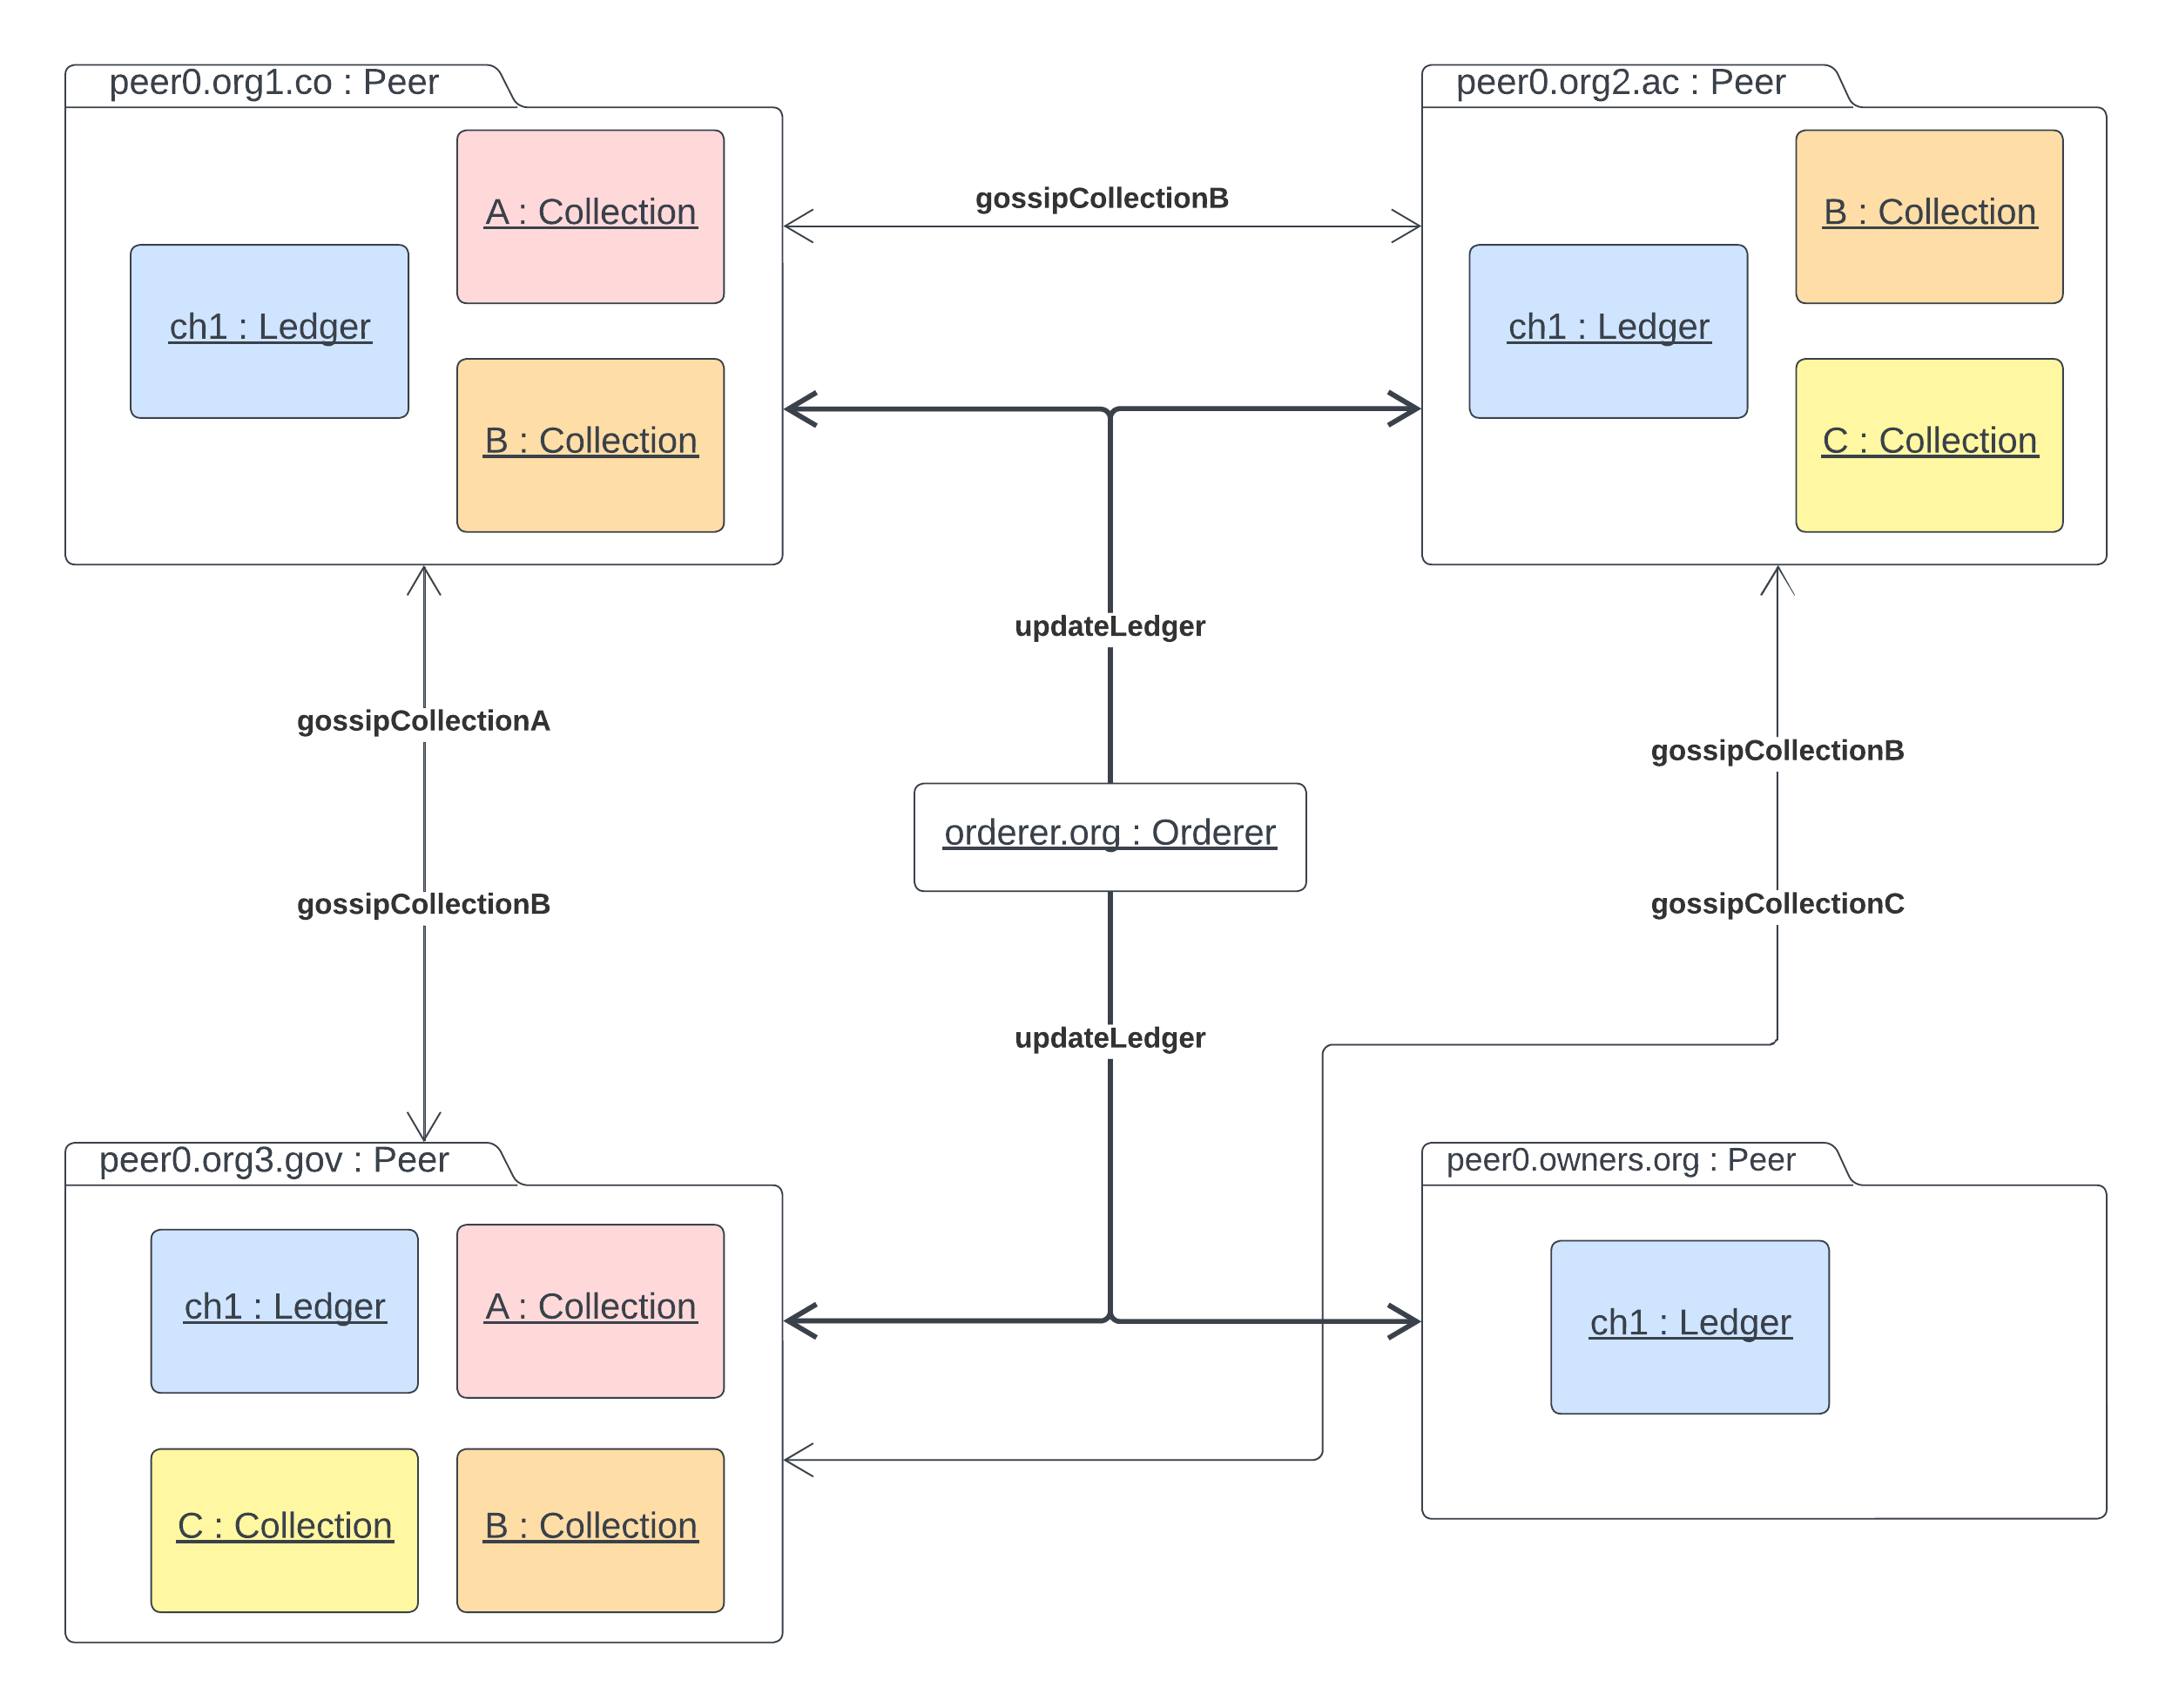
\includegraphics[width=\textwidth]{collections.png}
        \caption{A UML object chart showing a channel ledger and private collections}
        \label{fig:collections}
    \end{figure}

    \subsection{Data publishing and consent preservation}
    Data in this system can be stored two ways - either in public ledger or replicated private collections. For both methods, LevelDb database is utilised. To store or read a value, it needs to be identified by a key, which can be composite and identify more than one quality of the value. Chaincode is used to access ledger or private collections with a key and any change is expressed as part of an invoke transaction. All non-empty public ledger keys make up a world state, which can always be reconstructed following every validated transaction. Changes to private collections are not reflected on the ledger - to keep sensitive information private. However, for the ability to confirm correctness of collection values, SHA-256 hash of every private value is published to the ledger. This way sensitive information is kept private, while the evidence of the new value is recorded.
    
    Two types of values are stored in a world state - table indices and consent constraints. Constraints reference a table index and a tuple of its columns that are not allowed to store in its entirity. For example, if a constraint is a combination of columns \lstinline{a} and \lstinline{c} in a table named \lstinline{T}, the consent constraint query would look like this: \lstinline{T(a,c)}. Chaincode flow dictates that a constraint must reference an existing table, meaning a table needs to be created first. Table has a name and a complete list of columns (an index), both of which cannot be changed. The syntax defining a table is the same as a constraint: \lstinline{T(a,b,c,d)}. Any information published to the table has to conform to the column format, so when using the above defined constraint and index to store a row of table \lstinline{T}, only columns \lstinline{a}, \lstinline{b} and \lstinline{d} will be saved to the system. When saving information, one out of three private collections also needs to be selected - meaning a different table with the same name can exist in all three collections. When creating a table index and setting constraint queries, no collection needs to be specified, so constraints related to a certain table will be applied to values in all collections. The semantics to express both a table index and a consent constraint is taken from \cite{konstantinidis}, where more complex semantics of consent are also defined, such as constraining a column from a union of tables. Here, only constraints of tuples from the same table are implemented. However, implemented system applies no limitations for constraint expressiveness, leaving the ability to implement the rest of the consent semantics in the future.

    \begin{figure}[H]
        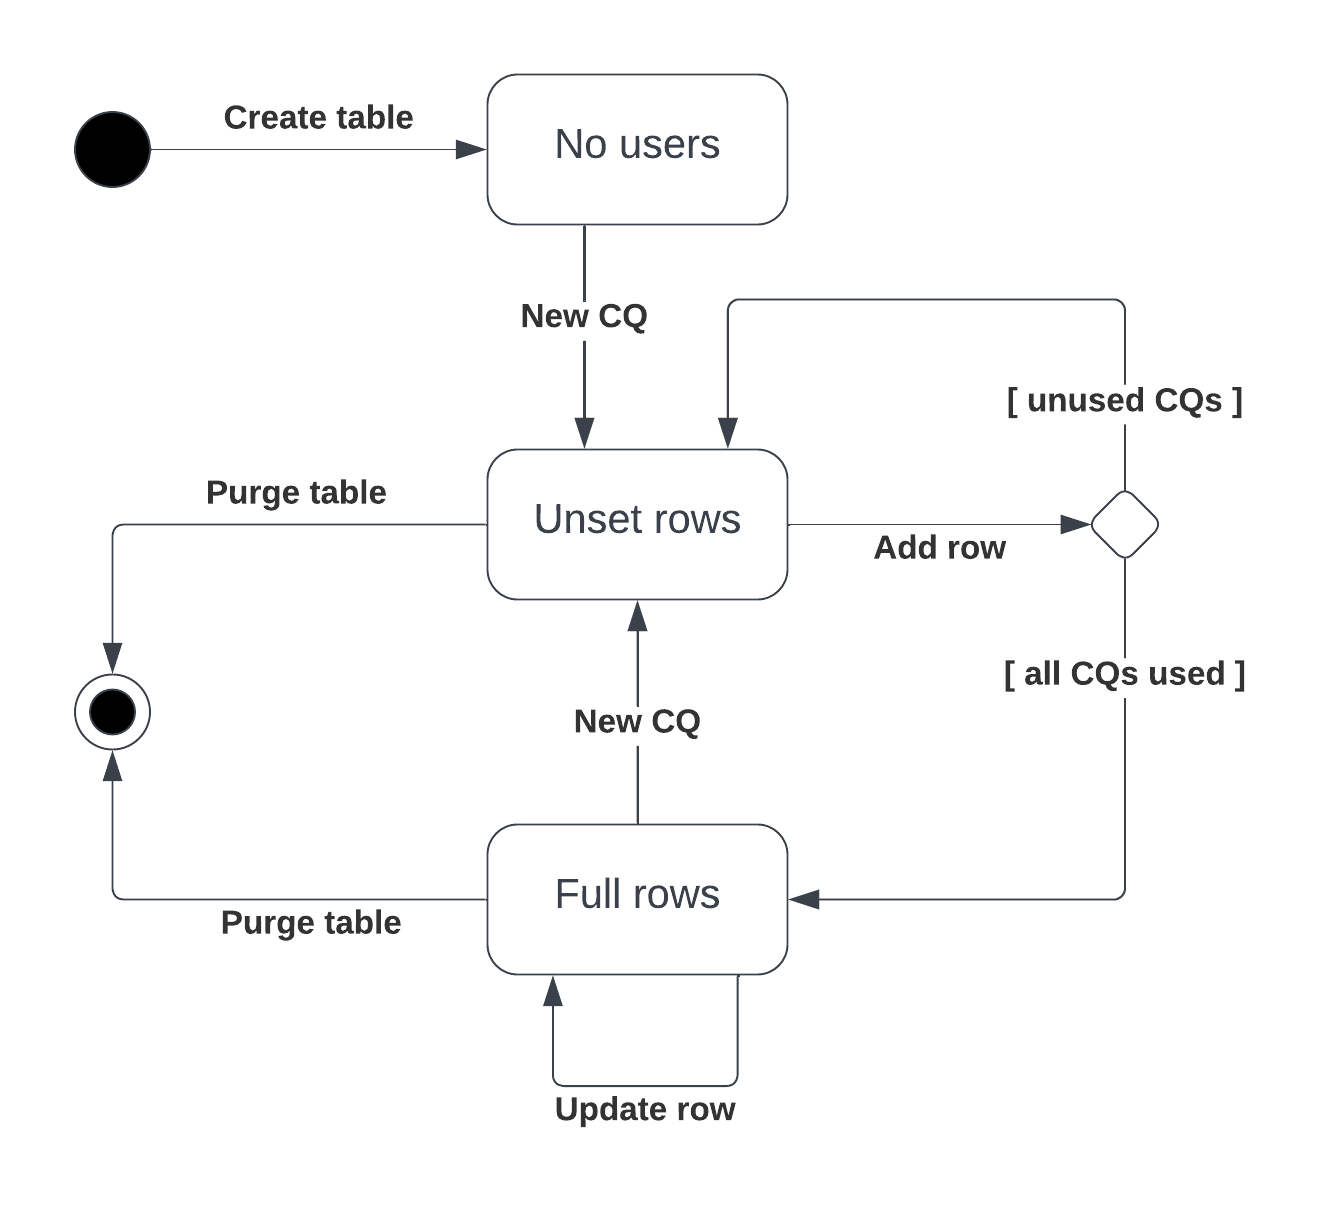
\includegraphics[width=\textwidth]{worldstate.png}
        \caption{A UML state diagram showing possible states of a table}
        \label{fig:worldstate}
    \end{figure}

    From the description above, table is a value related to one key in a single private collection. In figure \ref{fig:worldstate}, three possible table states can be seen. Any function can be invoked from any table state, but only functions marked as transitions in the state diagram can move table state to the next one. All chaincode functions can be found in appendix \ref{appendix:functions} with \lstinline{@Transaction} signature, while some functions are summarised to the bullet list below:

    \begin{itemize}
        \item First state can only be reached by creating an empty table. System chaincode implements function \lstinline{CreateTable(String)}, where a table definition, described above, is used to describe table columns. This definition is saved to the ledger with a table name as a prefixed key to indicate this is a table value.

        \item As seen in the state diagram, there is no way to submit a user constraint or upload user data without creating a table first, which is a result of a condition in function \lstinline{SetConstraint(String)}. This function accepts consent constraint query of format described above as input, checks if a table exists, and only then saves the constraint definition to the ledger. This check prevents users from submitting their constraints to a table that does not exist and does not have its index defined.
        
        \item With a set constraint, table moves into a state of unset rows - meaning there are users that have submitted consent for this table and their data is yet unpublished. Function \lstinline{UpdateTable(String, String)} can be invoked to append new user rows to the table. This function is where user constraints are used to filter user data being published. Input data is passed as transient data - function input that does not get saved to a transaction. Destination private collection and an update query - tuple defining which columns are updated - are passed as parameters. After completing the function, world state does not change, but specified private collection gets updated with filtered user information and transient data is discarded from endorsing peers, leaving no trace of private information in the system.
        
        \item When all CQs (constraint queries) have been used to update table rows, all users have their data published on the table. To add new users, more consent constraints have to bet set. Otherwise, update function can only be used to update existing rows while rejecting data of new users. Because this system is designed to deal with sensitive information, an option to purge personal information is essential. Hyperledger Fabric private collections satisfy this requirement by allowing purging values from all replicated collections. This functionality is exposed via function \lstinline{PurgeTable(String, String)}, which accepts collection name and table name as parameters. If table data exists in more than one collection, this function would require invoking for each collection. For this implementation, any member of specified collection can purge table data. In production implementation, this function would be better protected, but it is not in the scope of this project.
    \end{itemize}

    These chaincode functions implement the state diagram displayed in figure \ref{fig:worldstate}. In this model, data subjects have complete control over their data to be published onto the system. This model, however, does not control data that is already published, meaning stricter user consent would not erase past information, which was published under more open constraints. This implementation choice was done to preserve simplicity, as separate row purging would require the usage of CouchDb, instead of lightweight LevelDb.


    \subsection{Chaincode invokation}
    % identities
    As mentioned in subsection \ref{subsec:network}, four organizations are defined in this system. To interact with the network, an identity corresponding to one of the organizations needs to be issued. In Hyperledger Fabric, this task is done by Certificate Authorities (CAs) of each organization. User certificate issued by their organization CA is used to correctly evaluate access to information published in the system. When setting consent constraints, unique user address defined in the certificate is used to set apart one user's constraints from another. Likewise, when updating and querying private data, identity is used to confirm the collection for private data is accessible to the user. Identities also have roles and an identity with a role of \lstinline{admin} exists for every organization, which is used to issue other identities of the same organization. Users consenting to share their data can only set constraints with an identity of \lstinline{Owners} organization. This makes setting a constraint independent from publishers and gives the ability to issue data subject identities related to existing identification systems, such as email address, insurance number or a bank account, however, this topic is out of scope for this project. Identities of publisher organizations would be given out for private data access, with organization scope permissions regulating what information can different identities access.

    % fablo rest
    Fablo provides a simple REST interface for identity issuing and chaincode invokation with endorsement. This is a Node.js server application with endpoints to enroll identities and interact with chaincode, and each organization has an instance of this application. Using admin identity, a new org member can be enrolled - in that case, both the admin and the user can invoke chaincode, although may have different access rights. The application uses Fabric Gateway API to communicate with the Fabric network, which can be integrated into any computer program, making registering to an organization and interacting with the system available for everyone. Furthermore, each organization can decide how their Fabric Gateway application should behave, who should be given access to it and how to manage organization identities.

    \begin{lstlisting}[style=http,
        caption={HTTP requests to issue Owners identities and set constraints}, label={lst:invoke}]
> POST /user/register
> Authorization: Bearer admin-token
> {"id": "user", "secret": "userpw"}
200 OK

> POST /user/enroll
> {"id": "user", "secret": "userpw"}
200 OK
Authorization: Bearer user-token

> POST /invoke/ch1/private-data
> Authorization: Bearer user-token
> {
>   "method": "SetConstraint",
>   "args": ["T(a,c)"]
> }
200 OK
{"response": "Constraint set successfully"}

> POST /query/ch1/private-data
> Authorization: Bearer user-token
> {
>   "method": "GetTableConstraints",
>   "args": ["T"]
> }
200 OK
{"response": "{user=T(a,c)}"}
    \end{lstlisting}

    Listing \ref{lst:invoke} shows HTTP requests and responses from \lstinline{Owners} Fabric Gateway application. The objective of these requests was to register a new user and set their consent for table \lstinline{T(a,b,c,d)}. First request is authorized by an enrolled admin wanting to register a new organization identity. After registration, user can utilize new identity by enrolling with a user id and a secret. After enrolling, authorization token is used for further network interaction. Two chaincode functions are called using different Fablo REST endpoints. Function \lstinline{SetConstraint(String)} writes a new constraint to the ledger, therefore a transaction must be produced to invoke chaincode function, using \lstinline{\invoke} endpoint. \lstinline{GetTableConstraints(String)} can be called without producing endorsement transaction - for this reason \lstinline{/query} endpoint is used.


    \section{Testing and evaluation}
    This project has discovered many decision points when designing and implementing a trustless information exchange. Some decisions have altered performance of the system and can be measured and compared. Other design decisions are functional, creating new features improving privacy, reliability and user data ownership. This section will test functional features of the system, evaluate and compare performance metrics to other information exchanges. Scenario testing will be performed on the implementation of the system, assessing the degree of trust required, decentralisation benefits and transparency of the blockchain. Transaction speed evaluation will enable to compare the performance cost of user consent preservation algorithms to an information exchange.

    \subsection{Scenario testing}
    \label{sec:scenario}
    
    % describe current state, referrence sec:implementation 
    % - 3 orgs, owners
    % - installed cc in append A
    % - enrolled to the network with all necessary accs
    
    % complete transactions and observe the information of the system:
    \begin{table}[ht]
        \footnotesize
        \begin{tabular}{ c|c|c|c|p{0.15\linewidth} }
         identity & function & atom & collection & transient / response \\
         \hline
         admin@org3.gov & UpdateTable & T(disease,age,hospital) & C & user,cancer, 46,stmarys
        \end{tabular}
    \end{table}

    % - what got published ?
    % - how efficiently has the data been communicated ?

    % - how much user had control over their data ?
    % - what parties did we trust in the process ?

    % - try disconnecting one of peers

    \subsection{Evaluation}

    \subsection{Future considerations}
    % not enough time for this - what took longer to do?
    \label{sec:future}



    \section{Conclusion}


    
    
    \newpage
    \bibliographystyle{ieeetr}
    \bibliography{refs}


    \newpage
    \appendix
    \section{Appendix: Chaincode functions}
    \label{appendix:functions}

\end{document}
